\documentclass[11pt,a4paper]{article} 

\usepackage[T1]{fontenc}
\usepackage[utf8]{inputenc}
\usepackage{lmodern}
\usepackage[french,english]{babel}

\usepackage{amsthm}
\usepackage{float}
\usepackage{lmodern}%pour un meilleur rendu des polices
\usepackage{verbatim}%du texte non interprt
\usepackage[cmex10]{amsmath}
\usepackage{amssymb}%maths
\usepackage{xspace}
\usepackage[dvipsnames,svgnames,table]{xcolor}
\usepackage{listings}
\usepackage{fancyhdr}
\usepackage{etoolbox}
\usepackage{titlesec}
\usepackage{titletoc}
\usepackage{lastpage}
\usepackage[bookmarks=true,bookmarksnumbered=true]{hyperref}
\usepackage{ctable} % for \specialrule command
\usepackage{cite}
\usepackage{algorithm2e}
\usepackage{alltt}
\usepackage{array}
\usepackage{mdwmath}
\usepackage{mdwtab}
\usepackage{eqparbox}
\usepackage[caption=false,font=normalsize,labelfont=sf,textfont=sf]{subfig}
\usepackage{dblfloatfix}
\usepackage{url}
\usepackage{tipa}
\usepackage{stmaryrd}
\usepackage{multirow}
\usepackage{adjustbox}
\usepackage{subcaption}
\usepackage{subfig}

%\usepackage{natbib}
%\usepackage[pdftex]{graphicx}
%\usepackage{framed}
%\usepackage[usenames]{color}

\graphicspath{{img/}}
\DeclareGraphicsExtensions{.pdf,.jpeg,.jpg,.png}

%% taille du papier
\textwidth 16 true cm
\textheight 24 true cm
\addtolength{\hoffset}{-1.5cm}
\addtolength{\voffset}{-1.5cm}

%-------- couleurs
\definecolor{grisf}{rgb}{.47,.47,.47} % barre de droite gris fonce
\newcommand{\colorc}{\color{MidnightBlue}}
\newcommand{\colorb}{\color{NavyBlue}}
\newcommand{\colora}{\color{Cerulean}}

%----------- sections et TOC
% chapitres
\titleformat{\chapter}[display]
  {\normalfont\sffamily\bfseries\huge\colora\centering}{\thechapter}{1ex}
  {{\titlerule[1pt]}\vspace{1.3ex}}[\vspace{1ex}{{\titlerule[1pt]}}]
  
% chapitres etoiles  
\titleformat{name=\chapter,numberless}[display]
  {\normalfont\sffamily\bfseries\LARGE\colora\centering}{}{1ex}
  {{\titlerule[1pt]}\vspace{1.3ex}}[\vspace{1ex}{\titlerule[1pt]}\vspace{2ex}]
  
% sections  
\titleformat{\section}[hang]{\Large\normalfont\sffamily\bfseries\colora}{{\thesection\, }}{0 em}
  {}[{\titlerule[1pt]}\vspace{1ex}]

  
% sous section, sous sous sec, paragraphes  
\titleformat{\subsection}[hang]{\Large\normalfont\sffamily\bfseries\colorc}{{\thesubsection\, }}{0 em}
  {}[{\titlerule}\vspace{.7ex}]
\titleformat{\subsubsection}[hang]{\normalfont\sffamily\bfseries\large}{{\thesubsubsection\, }}{0 em}
  {}[{\color{grisf}\titlerule}\vspace{3pt}]
\titleformat{\paragraph}[runin]{\normalfont\sffamily\bfseries\colorb}{}{0 em}
  {\indent}



%----------------- fancy headers -------------%

\makeatletter
\patchcmd{\@fancyhead}{\rlap}{\color{grisf}\rlap}{}{}
\patchcmd{\headrule}{\hrule}{\color{grisf}\hrule}{}{}
\patchcmd{\@fancyfoot}{\rlap}{\color{grisf}\rlap}{}{}
\patchcmd{\footrule}{\hrule}{\color{grisf}\hrule}{}{}
\makeatother

                                                                    
\fancyhf{}
\fancyhead[R]{\sffamily Article summary }
\fancyfoot[R]{\sffamily\small{\thepage/\pageref{LastPage}}}
\fancyhead[L]{\sffamily\small{Jean-Baptiste Keck}}
\fancyfoot[L]{\sffamily\small{M2 MSIAM -- Optimal Transport - Levelset  -- 2014-2015}}
\renewcommand{\headrulewidth}{0.2pt} %0.4
\renewcommand{\footrulewidth}{0.2pt} %0
\addtolength{\headheight}{0.pt}

\fancypagestyle{plain}{
  \fancyhead{}
  \renewcommand{\headrulewidth}{0pt}
  }
     
  %-- macros --%   
  \def\hlinewd#1{%
      \noalign{\ifnum0=`}\fi\hrule \@height #1 %
  \futurelet\reserved@a\@xhline} 

  %------------------- front page ------------------%
  \title{
      \bsc{Paper Review}
      \vskip 1cm
      {\colorb\textbf{Texture Mapping via Optimal Mass Transport}}
      \vskip 1cm
      {\colorc\textit{Ayelet Dominitz and Allen Tannenbaum}}
      \vskip 1cm
      {IEEE Visualization and Computer Graphics 2010}
  }
\author{%
    Jean-Baptiste \bsc{Keck}
    \vskip 0.5cm
    \bsc{M2 Msiam}
}
%\date{27 janvier 2014}
\makeatletter

\def\maketitle{%
    %\thispagestyle{empty}%
    \begin{flushleft}
        \normalfont\LARGE\par
    \end{flushleft}
    \vskip 2cm
    \begin{center}%
        {\colora\specialrule{.2em}{0em}{0em}}
        \vskip 1cm
        {\Huge \@title}%
        \vskip 1cm
        {\colora\specialrule{.2em}{0em}{0em}}
        \vskip 4cm
        {\Huge \@author\par}%
        \vskip 2cm
        {\Huge \@date\par}%
        \vskip 1cm

    \end{center}%
    \clearpage
}

\newcommand{\ccite}[1]{\textbf{\cite{#1}}}
\newcommand{\pd}[2]{\dfrac{\partial #1}{\partial #2}}
\definecolor{lightgray}{gray}{0.9}
\renewcommand{\colbox}[1]{\colorbox{lightgray}{$ #1 $}}
\renewcommand{\norm}[1]{\lVert #1 \rVert}
\renewcommand{\det}[1]{\lvert #1 \rvert}
%%%%%%%

\begin{document}
\pagestyle{fancy}

\maketitle

%\tableofcontents
%\clearpage

\section{Introduction}

Texture mapping is a method for adding detail, surface texture, or color to a computer-generated graphic or 3D model. 
In order to do this, texture coordinates have to be specified at each vertex of a given triangle. This can be seen as a mapping between the texture and the 3D model mesh. The whole difficulty is to find an optimal mapping in such a way that original texture geometry and patterns are kept.
This paper exposes a new method to compute such a mapping were the resulting mapping is area preserving and minimizes angle distortion in an optimal mass sense.

\section{The texture mapping problem}

Texture mapping is the 3D modeling process of making a 2D image representation of a 3D model's surface.
This process is also called uv-mapping where $u$ and $v$ denotes the axes of the 2D texture (because $x$, $y$ and $z$ are already used to denote the axes of the 3D object model space).
UV-texturing permits polygons that make up a 3D object to be painted with color from an image, an uv-texture map.
The uv-mapping process involves assigning pixels (or texels) in the image to surface mappings on the polygon, which is usually done at the end of the rendering pipeline in the fragment shader.

\vskip 0.3cm
\begin{figure}[H]
   \centering
   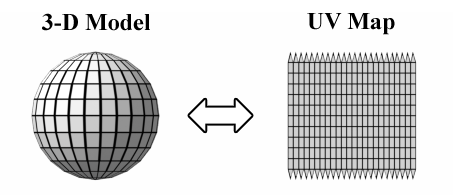
\includegraphics[width=8cm]{1.png}
   \caption{uv-mapping}
\end{figure}
\vskip 0.3cm

\subsection{On a sphere}

Let $S^2$ be the usual sphere. Finding a mapping from the texture to the sphere is an easy problem and can be done by equirectangular projection. 

\vskip 0.3cm
\begin{figure}[H]
   \centering
   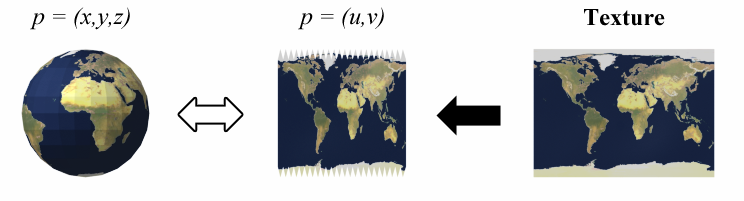
\includegraphics[width=12cm]{2.png}
   \caption{uv sphere mapping}
\end{figure}
\vskip 0.3cm

The equirectangular projection maps the longitudes and latitudes directly into the $u$ and $v$ coordinates on the plane, respectively. The poles (zenith, nadir) are mapped to the top and bottom edges and are stretched to the entire width of the image. Areas near the poles get stretched horizontally. This projection is easy to use because of the simple connection between the pixel coordinates on the plane and its azimuth and zenith angles on the sphere. However, it is neither area preserving nor angle preserving.

\vskip 0.3cm
\noindent Assuming the poles are aligned with the $y$-axis we directly have with normal coordinates:

$$
\colbox{
\begin{array}{l c l c c c l c l}
    u & = & 0.5 + \dfrac{arctan2(n_z, n_x)}{2\pi} &
    &&&
    v & = & 0.5 + \dfrac{arcsin(n_y)}{2\pi}\\
\end{array}
}
$$

\subsection{On a general closed surface}

The problem is that every surface is not a sphere... But they might be topological spheres if the surface $\Omega$ is \textbf{compact} and \textbf{simply-connected}. In other words a surface is a topological sphere if it is a closed surface and if there is no holes going through of it.

\vskip 0.3cm
\begin{figure}[H]
   \centering
   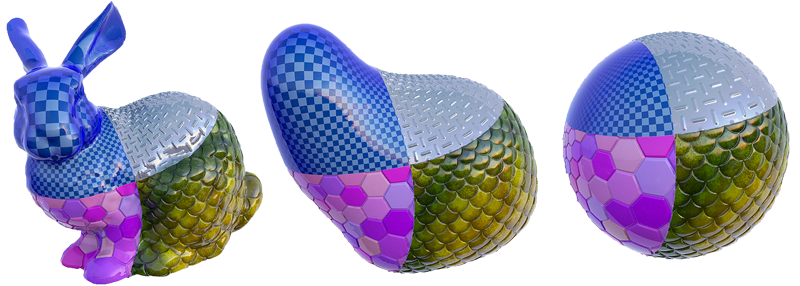
\includegraphics[width=12cm]{3.png}
   \caption{Example of topological sphere : The Stanford Bunny}
\end{figure}
\vskip 0.3cm

This implies that $\exists\ F : \Omega \to S^2$ such that F is a \textbf{diffeomorphism}.
With such a surface one could consider the \textbf{new problem} of finding an optimal mapping $F : \Omega \to S^2$ and then using $F^{-1}$ to directly paint the surface with any texture defined over $S^2$ or using last paragraph uv-sphere texturing for any texture.

\section{Existing methods}

Finding such an optimal mapping $F$ between the sphere $S^2$ and the surface $\Omega$ has been a major concern in the last decades.

\vskip 0.3cm

In general, there may be several natural measures for the goodness of the mapping. 
From one point of view, we wish to obtain a mapping that preserves the local geometry of the original
surface and this can be obtained using a \textbf{conformal mapping}.

\vskip 0.3cm

On the other hand, it is reasonable to require the mapping to be \textbf{area preserving} to preserve texture scaling.

\vskip 0.3cm

However, in general, it is \textbf{not possible} to map a simply connected compact surface with non-constant Gaussian curvature to the sphere in a way that preserves both angles and areas. In fact it is only possible if $\Omega$ is a usual sphere too.

\subsection{Area Preserving Mapping}

Area preserving mappings constitutes the first great family of optimal mappings. It is optimal in the sense that it preserve local areas.

\vskip 0.3cm
In fact, with $\mathcal{A}$ a given measure, a map $F:\Omega \to S^2$ is area preserving if and only if:
$$\colbox{\forall K \subset \Omega\ \ \mathcal{A}(K) = \mathcal{A}(F(K))}$$

\begin{figure}[H]
   \centering
   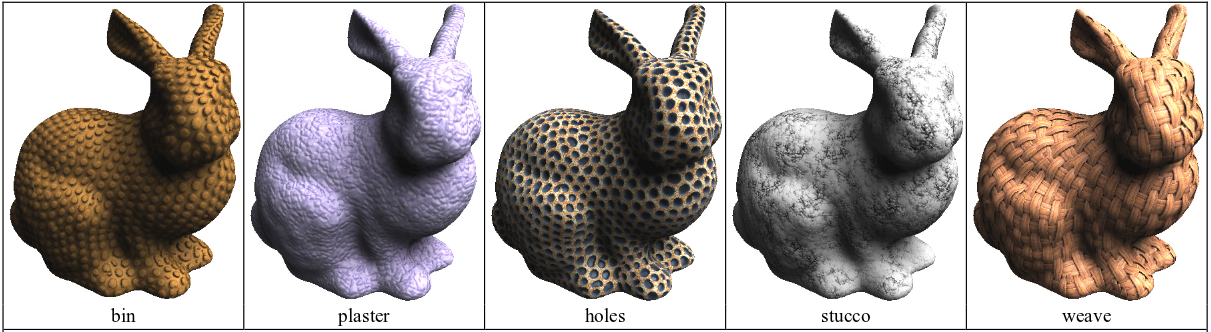
\includegraphics[width=16cm]{4.png}
   \caption{Examples of area preserving texturing}
\end{figure}
\vskip 0.3cm

\textbf{This mapping preserves local area but is not unique} and causes geometric deformations.

\subsection{Conformal Mapping}

Conformal mapping, angle-preserving mapping or biholomorphic mapping constitutes the second family of optimal mappings. It is optimal in the sense that is preserves magnitude and orientation of angles.

\begin{figure}[H]
   \centering
   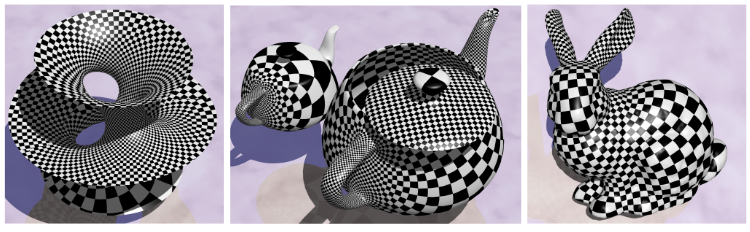
\includegraphics[width=16cm]{5.png}
   \caption{Examples of angle preserving texturing}
\end{figure}
\vskip 0.3cm


\textbf{This mapping preserves local geometry and is unique up to a Möbius transformation} (which transforms spheres into spheres) but causes stretching and shrinking on curved object.

\section{Proposed method}

The proposed method allows to find an optimal area preserving mapping $F$ from a general simply connected compact surface $\Omega$ to the usual sphere $S^2$. We can then use the inverse mapping $F^{-1}$ to paint the surface with any texture defined on the sphere.

\vskip 0.3cm

For the sake of simplicity we assume that the total surface area of $\Omega$ has been normalized, $ie.\ \colbox{\mathcal{A}(\Omega) = \mathcal{A}(S^2) = 4\pi}$. 
If not we have to consider non conservative mass transport like we have seen in the course extensions.

\vskip 0.3cm
\textbf{Here are the steps to extract optimal mapping $\colbox{F : \Omega \to S^2}$ :}
\vskip 0.3cm

\begin{itemize}

    \item \textbf{Step 1:} Construct a conformal mapping $\colbox{f : \Omega \to S^2}$ with any existing algorithm. As we have seen, this is unique up to a Möbius transformation $ie. $ if $f'$ is another conformal mapping there exists some diffeomorphism $\colbox{\chi : S^2 \to S^2}$ such that $\colbox{f' = f \circ \chi}$.
    
    \item \textbf{Step 2:} From the conformal mapping f, define a density function $\colbox{\mu = \det{\nabla f^{-1}}}$ which represents area distorsions caused by $f$ (determinant of the Jacobian of $f^{-1}$). 
        We aim for a area preserving mapping so we want to optimally transport our density $\colbox{\mu : S^2 \to \Omega}$ to the uniform density $1$ everywhere on $S^2$. The penalty function used is the geodesic distance $\colbox{\Phi(\vec{x},\vec{y}) = arccos(\vec{x} \cdot \vec{y})}$. 

        \vskip 0.3cm
        We want to minimize $\colbox{M(g) = \displaystyle \int_{S^2} \Phi(x, g(x))\ \mu(x) \mathrm{d}x}$ with mappings $\colbox{g^t: (S^2,\mu) \to (S^2, 1)}$.
        $dx$ is the area form of the standard metric on the sphere $\colbox{r^2 \sin(\theta) \mathrm{d}\theta \mathrm{d}\phi}$.
        
        The gradient flow used to move $g^t$ is a bit complex : $\colbox{R_{+\pi/2}\ \vec{\nabla} \left( div \left[ R_{+\pi/2}\Phi_x(x, g^t(x)) \right] \right)}$
        with $\colbox{\Phi_x(\vec{x}, \vec{g}(\vec{x})) = \dfrac{ \vec{x} \times \vec{g}(\vec{x}) }{\norm{\vec{x} \times \vec{g}(\vec{x})}  }}$.

        In addition they incorporate a multiresolution scheme with spherical wavelets into the flow to compute solutions faster.
    
    \item \textbf{Step 3:} $\colbox{F = g^{+\infty} \circ f : \Omega \to S^2}$ gives an area preserving mapping from $\Omega$ to the sphere. We can use the inverse mapping $\colbox{F^{-1} = \left( g^{\infty} \circ f \right)^{-1}}$ to paint from the sphere to original surface. 
\end{itemize}

\begin{figure}[H]
   \centering
   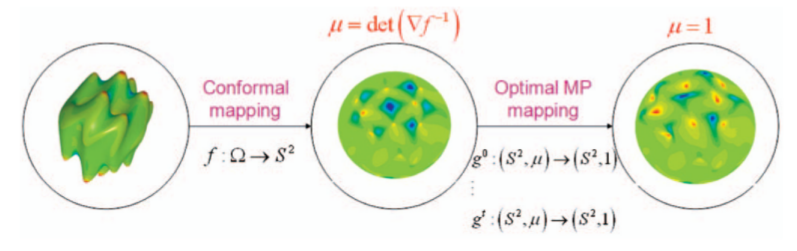
\includegraphics[width=16cm]{6.png}
   \caption{Block diagram of the algorithm}
\end{figure}
\vskip 0.3cm



\clearpage
\section{Results}

\subsection{Texturing comparison}

Here are the results of texturing with 3 conformal mapping techniques and the new method developed in this article :

\begin{figure}[H]
    \subfloat{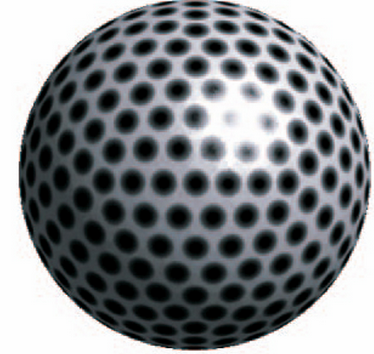
\includegraphics[width=.2\linewidth]{results1}} &
    \subfloat{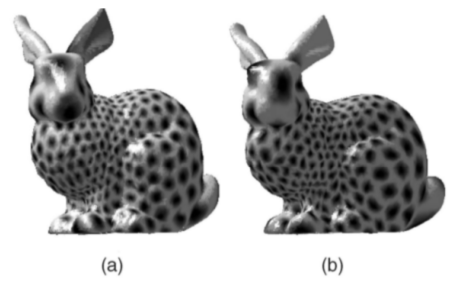
\includegraphics[width=.4\linewidth]{results1a}}&
    \subfloat{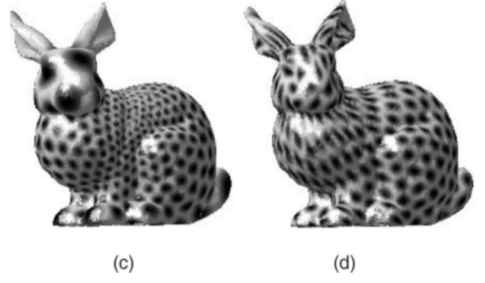
\includegraphics[width=.4\linewidth]{results1b}}
    \caption{Results for different techniques on the Stanford Bunny with given textured input sphere.\\
        \textbf{Conformal methods :} Gotsman et al[2] mean value(a) \& Tutte weights(b), Haker et al[3](c)\\
        \textbf{New hybrid method:} (d)}
\end{figure}

It is clear that the first tree ones do not try to preserve locally area and that the new one takes it in account. As local angles and areas are in some sense optimally mapped, the texture rendered with the new method seems more naturally distributed on the bunny which is exactly what this paper aimed at.

\vskip 1cm
\subsection{Mapping statistics}

Here are some metrics to compare their new method with existing conformal mappings and area preserving mappings :
\vskip 0.5cm

\begin{adjustbox}{center}
\begin{tabular}{| l || c | c | c || c || c |}
    \hline
    \multicolumn{1}{|c||}{Stanford Bunny} &  \multicolumn{3}{c||}{Angle preserving methods} & Area pres. methods & Hybrid\\ 
    \cline{2-6} \multicolumn{1}{|c||}{(70k triangles)} & \textbf{Saba (tutte)} & \textbf{Saba (mean)} & \textbf{Haker} & \textbf{Moser} & \textbf{New method} \\    
    \hline
    \textbf{Angular distorsion}  & 2.65 & 2.52 & 2.02 & 3.17 & 2.76 \\
    \hline
    \textbf{Area    distorsion}  & 3.47 & 3.65 & 3.26 & 2.57 & 2.66 \\
    \hline
\end{tabular}
\end{adjustbox}

\vskip 0.5cm
As the conformal method developed by Haker is the starting point of the optimal transport iterations, we really see how the metrics are evolving : Angular distorsion increases slightly but area distorsion is drastically reduced. In fact it is so much reduced that we can practically compare it to a fully area preserving method as the Moser algorithm but with incredible angle preserving capabilities. 

\clearpage
\subsection{Performance statistics}

Here are some metrics to check the computational cost of the algorithm :
\vskip 0.5cm

$$
\begin{tabular}{| l || c | c | c |}
    \hline
    \textbf{Model}  & \textbf{\# of faces} & \textbf{\# of iterations} & \textbf{time (s)} \\
    \hline
    Squirrel   & 5k & 814 & 971    \\
    \hline
    Max-Planck & 25k & 2120 & 2460 \\
    \hline
    Skull      & 40k & 1371 & 2132 \\
    \hline
    Bunny      & 70k & 2530 & 3093 \\
    \hline
\end{tabular}
$$

\vskip 0.5cm
Even with optimized multiscale spherical wavelet approach this algorithm seems pretty slow because of the optimal transport iterations. However there is no data concerning the other algorithms so we can not compare it to the others. 

\section{Conclusion}

In this paper was introduced a novel method for the parameterization of 3D objects. 
In the proposed method, the optimal mapping is an area preserving mapping produced via optimal mass transport of an original angle preserving mapping. 
The optimal mass transport map is found via a gradient flow directly computed on the sphere, implemented using a multiresolution scheme
for fast convergence. 
It is also shown that we can use the new method to map textures onto closed compact simply connected surfaces.
This new algorithm has been compared to results of other texture mappings derived from conformal and area preserving mapping theory.

\vskip 0.5cm
Personally I was convinced that their new method works as expected because the paper is really detailed with lots of examples and illustrations, everything is clear.
It is well structured and each part is clearly identified. Finally - and it is rare enough to deserve a mention - they included implementation considerations.
The thing I would have changed in this paper is to shorten the Related Work part 1.2 because it is really long with lots of references and it just adds little. The other little thing would be to better distribute the images and arrays within the paper instead of putting all these things on the 10 last pages !

\bibliographystyle{plain}
\bibliography{master}

\end{document}

